\section{Implement} %4.3

One of the most important idea to implement the testing environment is to modularise the function (Figure~\ref{4_3_code1}). We modularised our functions in a python file so we can import them as a library and call them directly (Figure~\ref{4_3_code2}). Additionally, it is necessary to remove hardcoded parameters so it is easy to change the parameters like start time, end time, prepared folder address and the list of generators (Figure~\ref{4_3_code2}).

Another noteworthy detail is we need to keep two significant digits (Figure~\ref{4_3_code2}) for kp, ki and time delay. It provides an unified format that helps exporting data into analytical algorithms.

The script to generate the feasible kp-ki-td parameters is automatic and well documented (Figure~\ref{4_3_code2}).

\begin{figure}[htbp]
\centering
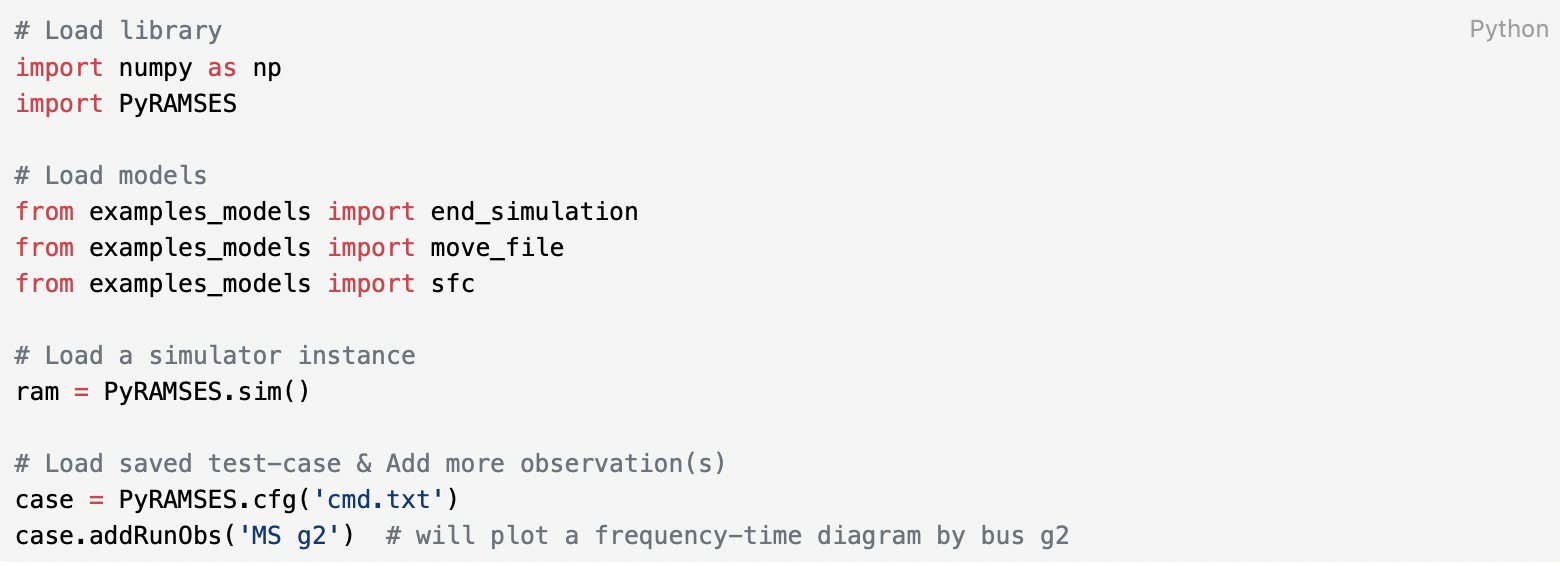
\includegraphics[width = \textwidth]{figure/4_3_code1.png}
\caption{Python: import related libraries.}
\label{4_3_code1}
\end{figure}

\begin{figure}[htbp]
\centering
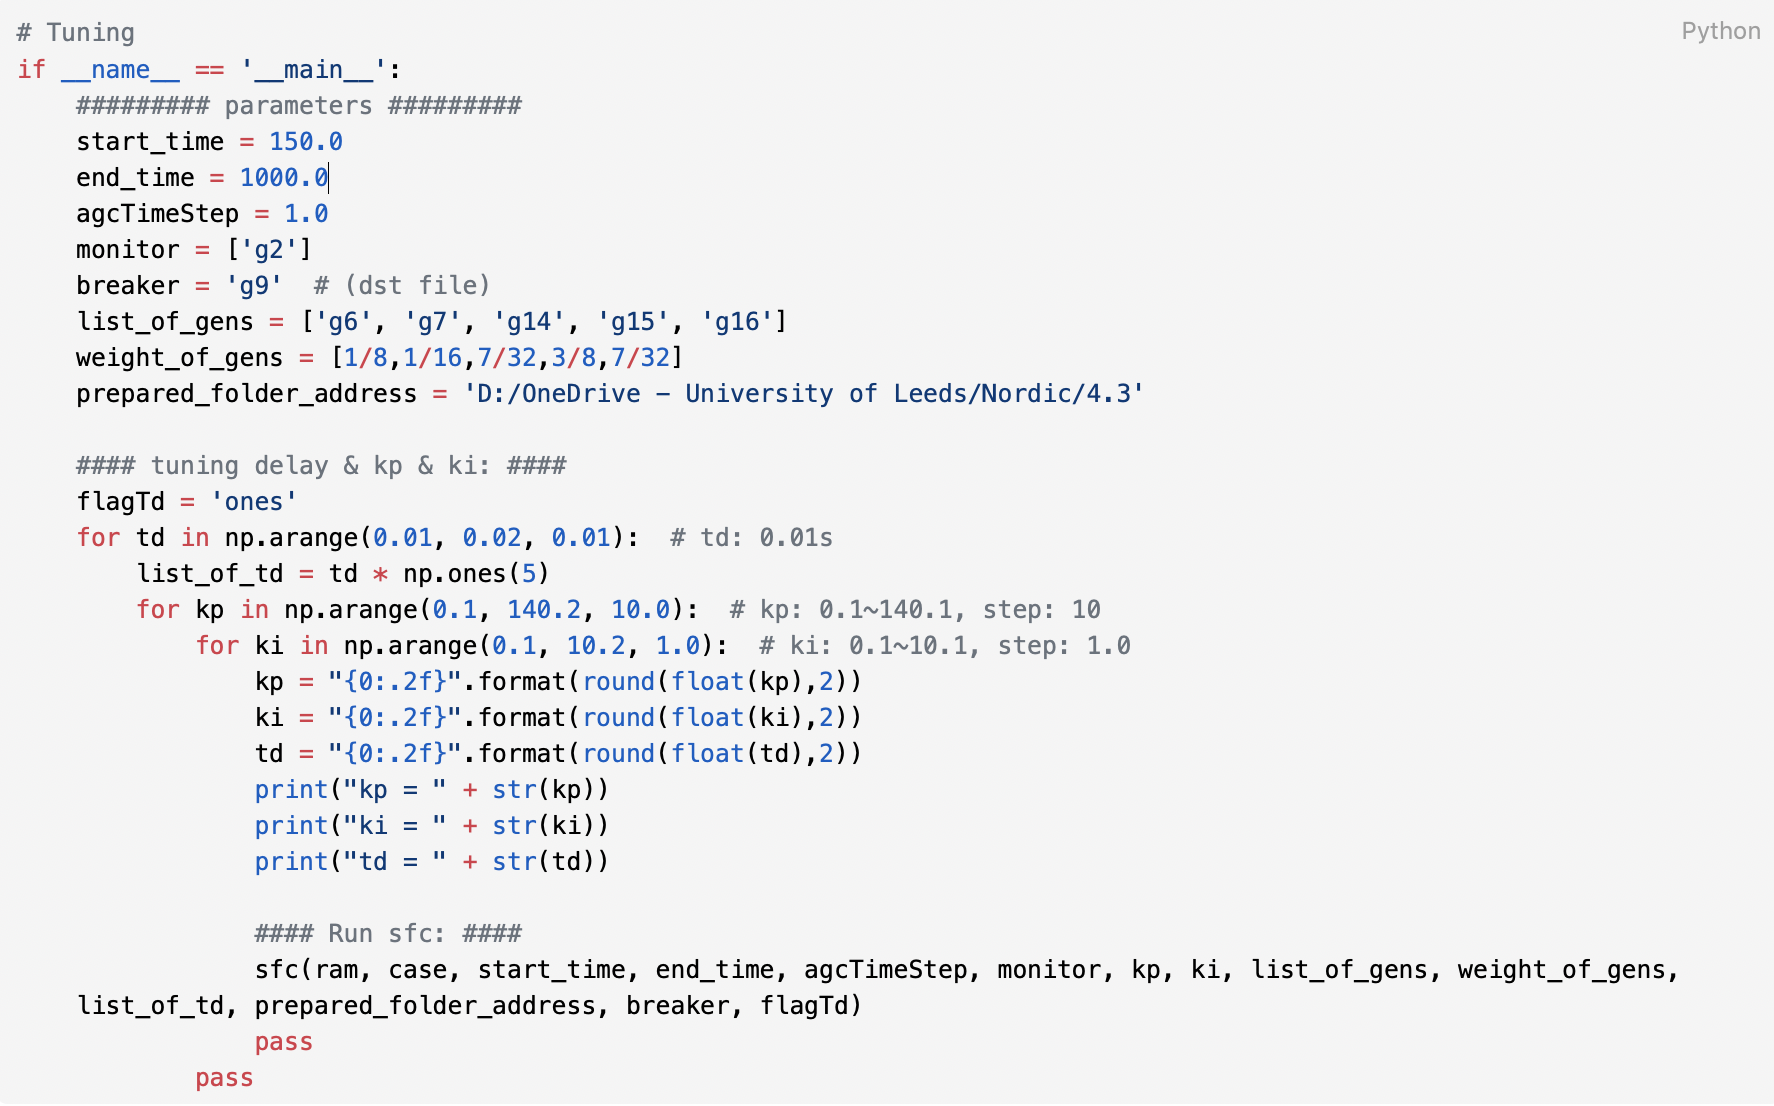
\includegraphics[width = \textwidth]{figure/4_3_code2.png}
\caption{Python: tune PI control.}
\label{4_3_code2}
\end{figure}